
\chapter{绪论}
\label{chap:introduction}

中国科学技术大学论文模板(ustcthesis)是按照中国科学技术大学学士、硕士和博士论文要求制作的\LaTeX 通用论文模板。其前身是中国科学技术大学本科论文模板(作者XPS,最后维护ywg)和中国科学技术大学研究生论文模板(作者Liuqs,主要维护Liuqs、Guolicai)。本模板在上述两模板基础上进行了整合梳理,将模板的基础实现和增强功能进行分离,分别提供最基础的ustcthesis.cls以及增强包ustcxtra.cls。其中,ustcthesis.cls仅提供模板的最基础格式,ustcxtra.cls则包含一些常用的优化设置及更为便捷的自定义命令。

本文是使用上述模板生成的示例文档,目的在于帮助使用者熟悉该模板的使用方法,并且为使用者学位论文的撰写提供基础代码示例。

\section{系统要求}
\subsection{系统要求}
本模板基于\CTeX 的ctexbook文档类进行定制,基于\XeTeX 引擎排版。使用本模板的最基础功能时,除了上述需求外,还需要如下几类宏包(直接引用):
\begin{description}
\item[数学类]{amsmath、amsthm、amsfonts、amssymb、bm}
\item[格式类]{titletoc、titlesec、geometry、caption}
\item[表格类]{multicol、multirow}
\item[其他]{xparse、xeCJK、hyperref、natbib、subfiles}
\end{description}
可能有部分宏包是由上述宏包以及\CTeX 间接引用的,此处不一一列举。

另外,如果需要使用增强的ustcxtra.cls,额外需要如下宏包(直接引用):
\begin{description}
\item[默认载入]{times、algorithm2e、graphicx、psfrag、subfig、enumerate、epsfig、float、paralist、booktabs、footmisc、wasysym、longtable、bbm、indentfirst、ifthen、caption3、array、fancyvrb、xcolor、url}
\item[条件载入]{eulervm(仅在文档类处于增强模式并在文档类选项注明euler时载入)}
\end{description}

\section{下载与安装}
\subsection{模板文件清单}
使用模板之前请确保模板文件没有缺失损坏。文件清单如\autoref{tab:filelist},标注关键的文件需要确保文件以及路径的完整。
\begin{table}[htp]
\centering
\tabcaption{模板主要文件清单}
\label{tab:filelist}
\begin{tabular}{lll}
\toprule
文件名&相对路径&备注\tabularnewline
\midrule
clean.bat			&./			&清理脚本\tabularnewline
clean.sh			&./			&清理脚本\tabularnewline
main.pdf			&./			&示例文件\tabularnewline
main.tex 			&./			&示例TeX文件\tabularnewline
make.bat			&./			&生成脚本\tabularnewline
make.sh				&./			&生成脚本\tabularnewline
ustcbib.bst		&./			&Bib格式文件\tabularnewline
ustcthesis.cls		&./			&(关键)模板\tabularnewline
ustcxtra.cls		&./			&(关键)模板增强\tabularnewline
ustc\_logo\_fig.eps	&./figures	&(关键)科大校徽\tabularnewline
ustc\_logo\_text.eps&./figures	&(关键)科大校名\tabularnewline
\bottomrule
\end{tabular}
\end{table}

\subsection{模板下载与使用}
由于Google公司决定停止Google Code服务,故原Google Code项目网站的模板整体迁移至GitHub网站并继续进行更新维护。本模板及本示例文件可以在GitHub网
站\url{https://github.com/ywgATustcbbs?tab=repositories}下载。备份托管地址为\url{https://gitlab.lug.ustc.edu.cn/ywg/ustcthesis},此托管网站由LUG@USTC提供服务。

请在项目页面选择ustcthesis->新页面中选择Download Zip下载最新模板文件(\autoref{fig:download})。也可以通过git clone的方式获得模板。

\begin{figure}
\centering
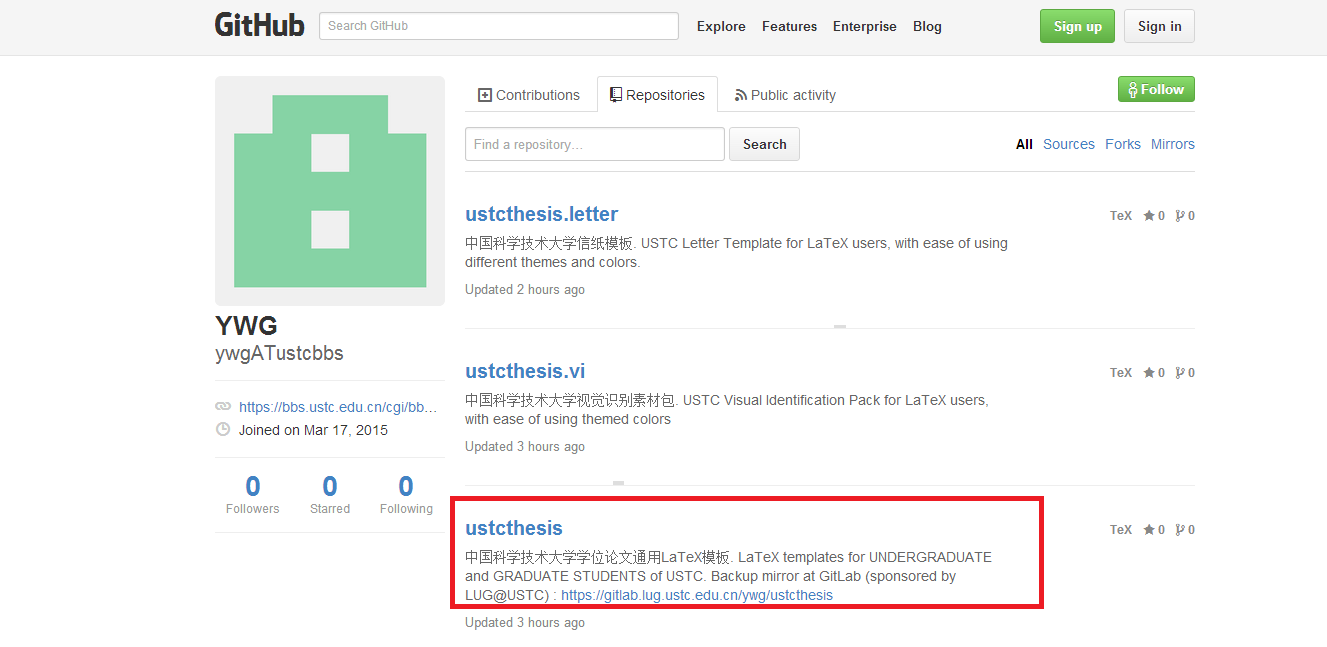
\includegraphics[width=0.48\textwidth]{download}
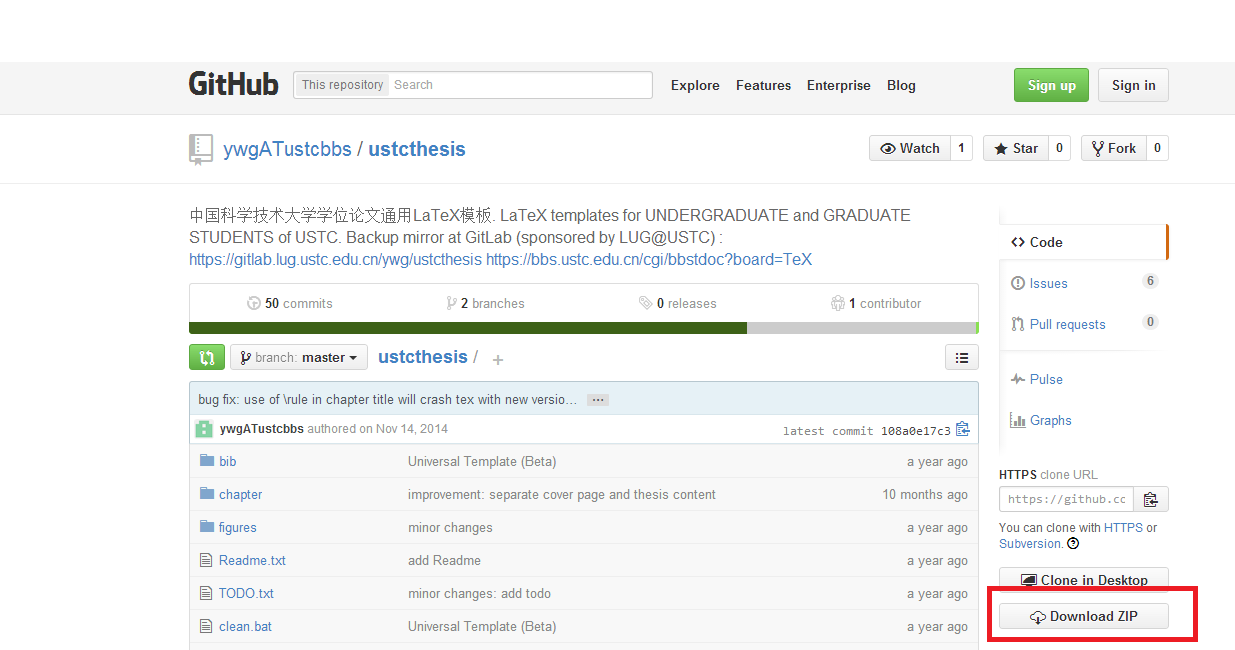
\includegraphics[width=0.48\textwidth]{download1}
\figcaption{在GitHub上进行模板下载}
\label{fig:download}
\end{figure}

\textbf{特别注意1:}本硕博通用论文模板的名称为ustcthesis,其他项目如ustcthesis.vi/ustcthesis.letter/ustcthesis.beamer是用作其他用途的模板,并非本模板所需文件,如对其感兴趣,请进入对应页面了解详情。

\textbf{特别注意2:}此前开发的本科和硕博模板已暂停支持,但仍然可以选择对应的版本(ustcthesis.bachelor和ustcthesis.msphd)进行下载。

模板的安装使用方法有多种,最为简单便捷的方法是直接解压缩下载好的压缩包,修改其中的main.tex文件以及chapter文件夹下的文件,必要时增加所需要的文件。需要注意的是确保所有文件使用UTF-8编码。Windows系统中将其他编码的文件转化为UTF-8的方法是: 用记事本打开这些文件, 然后点击文件—另存为—在最下方选择UTF-8 编码。

\subsection{\texorpdfstring{\LaTeX}{LaTeX}系统的安装和使用}
由于本模板使用了较多的宏包,因此建议使用TeXLive2013及以上版本的\LaTeX 发行版。TeXLive2013可以在Windows、GNU/Linux和大多数Unix系统中运行。对于MacOSX,推荐使用MacTeX-2013。详细信息参考\url{https://www.tug.org/texlive/}。

对于中国科学技术大学的校内用户而言,最方便的获取TeXLive2013的途径是使用LUG@USTC提供的CTAN镜像源(\url{http://mirrors.ustc.edu.cn/CTAN/})。最新的TeXLive位于/CTAN/systems/texlive/目录(\url{http://mirrors.ustc.edu.cn/CTAN/systems/texlive/})内。用户可以选择进入Images文件夹下载完整的光盘并刻录安装,也可以选择进入tlnet文件夹下载运行install-tl.exe进行在线安装。需要注意的是,在线安装的时候可以通过切换安装源为本校镜像源来加快下载安装速度。

对于校外用户,可以通过CTAN.org获得官方的TeXLive。CTAN在全球41个国家和地区分布有115个镜像站点,它们的地址可以在\url{http://www.ctan.org/mirrors/}找到。

\subsection{推荐使用的编辑器}
\LaTeX 的源文件是一个或多个文本文件,这意味着可以使用最为简单的文本编辑器来撰写论文。但是和许多编程语言类似,使用一款带有语法高亮、命令补全等功能的文本编辑器能够大大提升协作效率。

对于不同的编辑器而言,能够实现的功能也不尽相同,加之不同用户拥有不同的使用习惯,简单武断的说某一款编辑器好或者不好有失公允。对于\TeX 写作而言,用户使用的编辑器大致可以分为两类:通用的文本编辑器和专用的GUI编辑器。通用的文本编辑器中公认比较好用的有Vim(Linux)、Emacs(Linux)、Notepad++(Windows)等等\footnote{当然,这些软件可能都有跨平台版本,而且也有其他很多优秀的文本编辑器,不要在意这些细节啦,我并不想挑起编辑器的圣战。:P}。这些编辑器有着强大的功能,但是往往需要在编辑和编译之间来回切换。而专用的GUI编辑器如TeXShop(Mac)、TeXWorks(windows/Linux)和Winedit(Windows、付费软件)等虽然可能在文本编辑上略显笨拙,但是其优点在于编写和生成一体化,简单化。

使用何种编辑器这个问题见仁见智,但是对于一个刚从word转来的新人,从界面简洁、操作简单、功能实用的角度出发,TeXWorks不失为一款优秀的GUI软件,如\autoref{fig:texworks}。

\begin{figure}
\centering
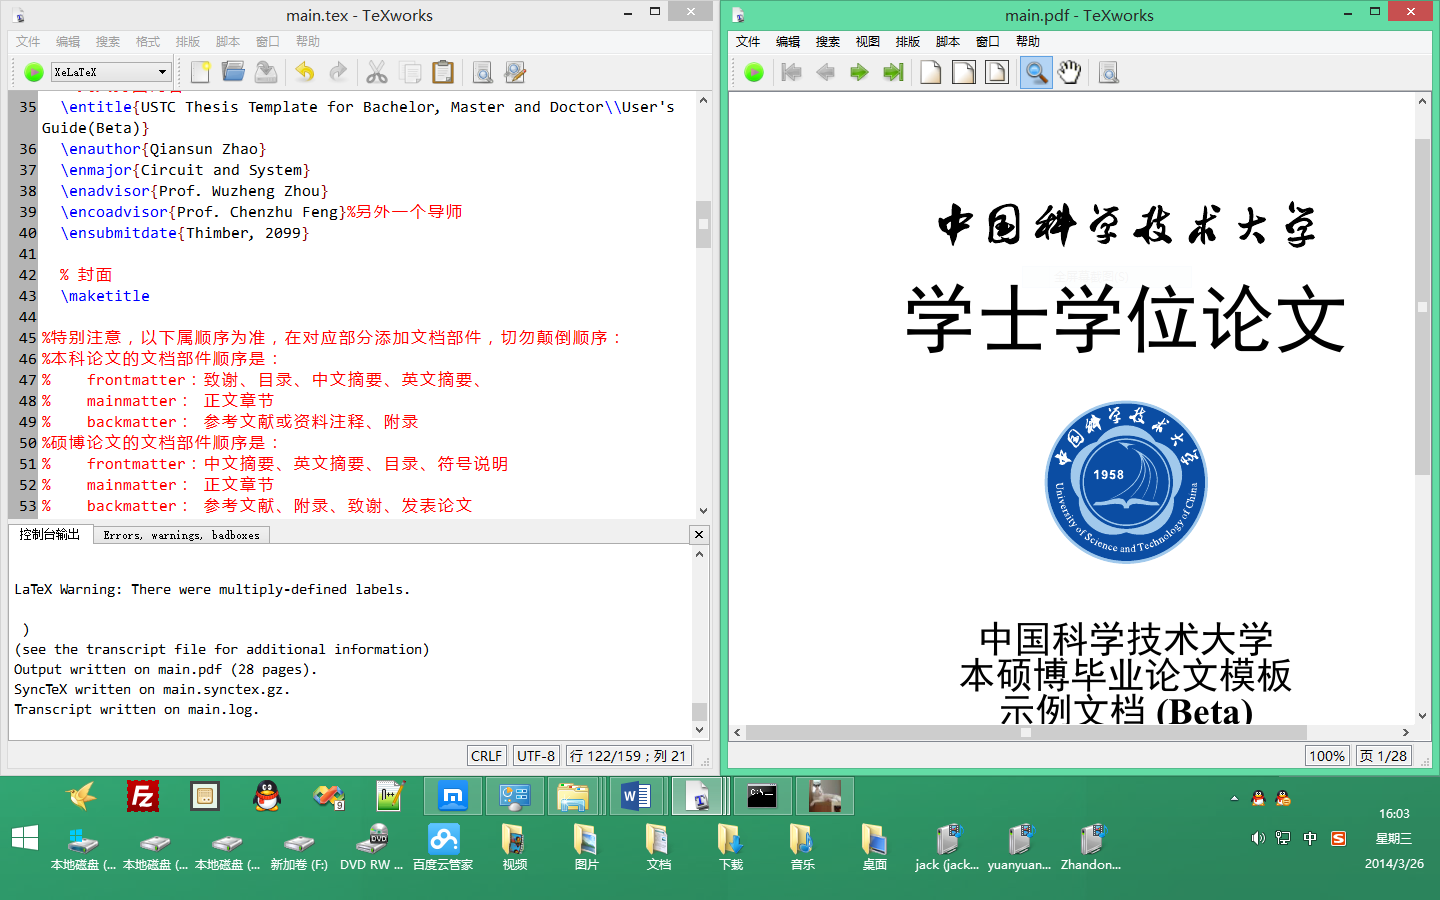
\includegraphics[width=0.9\textwidth]{texworks}
\figcaption{TeXWorks主界面}
\label{fig:texworks}
\end{figure}

Windows系统下TeXWorks的界面拥有左右两个窗口,左边为编辑窗口,右边为预览窗口,当编辑完文档之后,只需点击绿色的开始按钮,就可以立即对文档进行保存并编译,可以选择不同的引擎进行处理。编译过程中的信息会在左侧窗口下方显示。TeXWorks默认UTF-8编码,安装时自动查找TeX安装目录,支持自动缩进、语法高亮、命令补全、正则式查找以及TeX文件和PDF的正反查找(即点击命令跳转到对应pdf文字位置以及点击pdf文字跳转到对应命令,操作是Ctrl+单击)。这些功能对新手来说都是十分友好的。

\section{问题反馈}

如果您在使用过程中有疑问,遇到困难,可以在\href{http://bbs.ustc.edu.cn/cgi/bbsdoc?board=TeX}{瀚海星云\TeX{}讨论区}或者相关的\LaTeX 论坛(如\href{http://bbs.ctex.org}{CTEX 论坛})寻求帮助,但是请注意遵守论坛的各项规定。

如果使用过程中遇到Bug,请提交到\href{http://bbs.ustc.edu.cn/cgi/bbsdoc?board=TeX}{瀚海星云\TeX{}讨论区},或者提交到相应的\href{http://code.google.com/p/ustcthesis/issues/list}{Google UstcThesis Project(http://code.google.com/p/ustcthesis/issues/list)},请注明是什么版本模板的bug。